\documentclass[english,titlepage]{article}
%\documentclass[12pt,a4paper,titlepage]{article}
\usepackage{mathpazo}
\usepackage[T1]{fontenc}
%\usepackage[utf8]{inputenc}
\usepackage[a4paper]{geometry}
\geometry{verbose,tmargin=3cm,bmargin=3cm,lmargin=2.5cm,rmargin=2.5cm}
\pagestyle{plain}
\usepackage{authblk}


\usepackage{babel}

\usepackage{float}
\usepackage{textcomp}
\usepackage{amstext}
\usepackage{graphicx}
\usepackage{setspace}
\usepackage[authoryear]{natbib}
%\usepackage{cite}
\author[1]{Rebecca B Harris}
\author[2]{Christine Ewers-Saucedo}
\author[3]{Lucy M Li}
\author[4,5,6]{Julia A Palacios}
\author[7]{George Shirreff}
\affil[1]{Department of Biology, University of Washington, Seattle, WA 98122}
\affil[2]{Department of Evolution and Ecology, University of California at Davis, Davis, CA}
\affil[3,7]{Department of Infectious Disease Epidemiology, Imperial College London, London, W2 1PG, UK}
\affil[4]{Department of Organismic and Evolutionary Biology, Harvard University, Cambridge, MA, 02138}
\affil[5]{Center for Computational Molecular Biology, Brown University, Providence, RI 02912}
\affil[6]{Department of Ecology and Evolutionary Biology, Brown University, Providence, RI 02912}
%\usepackage[square,sort,comma]{natbib}
\date{}
\title{multiNe: the many facets of effective population size.}
\begin{document}
\bibliographystyle{molecol.bst}

\maketitle

\section{Abstract}
Inference of effective population size over time from genomic data is of paramount importance in a multitude of disciplines from conservation biology to epidemiology of infectious diseases. It provides insight about past evolutionary dynamics from present-day genomic data. [Something about different methods and sources of data to estimate the same thing and the motivation of this package] 
\section{Introduction}

A key parameter in elucidating the evolutionary history of a population is the effective population size over time $N_e(t)$, which is defined as the number of breeding individuals in an idealized population that show the same rate of genetic drift as the population being studied \citep{Wright1931}. Estimates of $N_e$ encompass the effects of both demographic and genetic processes in finite populations, thus effectively quantifying the rate and timing of molecular evolution \citep{Caballero1994}. Therefore, effective population size plays a central role in evolutionary studies seeking to disentangle the relative roles of stochastic and deterministic forces in modern studies of molecular evolution. Since then, it has become the primary parameter of concern for evolution, ecology, conservation biology studies and the surveillance of infectious diseases. 

Coalescent theory shows that under neutrality, effective population size trajectories on a completely linked segment of genomic data are separated by two stochastic process: an ancestral process that relates the samples (coalescent process of genealogies) and a stochastic process of mutations that acts on the branches of the genealogy of the sample. Despite its widespread usage in various disciplines, measuring $N_e$ in natural populations remains a challenge because the latent state space of genealogies grows exponentially with the number of samples and because $N_e$ is usually an unknown function (i.e. exponential growth or bottleneck) hard to parametrize in practice. Here, we simplify the problem by assuming that a representative genealogy is previously estimated and available. We extend current methods implemented in different \texttt{R}-packages such as \texttt{ape} and \texttt{phylodyn} to account for heterochronous sampling and multiple independent genealogies.

Alternatively, if we have reasons to assume that $N_{e}$ is constant over time, and our data consist of allele frequencies, we can assume a simple Wright-Fischer model. For example, neither linkage disequilibrium nor drift is expected in infinitely large populations, but both phenomena become more apparent as effective population size decreases. Thus by calculating the magnitude of linkage disequilibrium or genetic drift, we can infer $N_{e}$ if we know the mutation rate. Lacking mutation rate data, we can estimate $\theta$,  the mutation-rate scaled effective population size. $\Theta$ can be compared instead of $\N_{e}$ if we assume that mutation rates, albeit unknown, are comparable between systems. These Wright-Fischer estimators calculate Ne over the past few generations, whereas coalescent estimators integrate $N_e$ over the past $N_e$ to 4 * $N_e$ generations.

%More specifically, the product of the mutation rate and effective size $\theta$ can be estimated from summary statistics such as the number of segregating sites \cite{Watterson1975}, number of alleles \cite{Ewens 1972}, heterozygosity \citep{Kimmel1998}, and variance of the number of microsatellite repeats \citep{Kimmel1998}. Alternatively, $\theta$ can be estimated from the genealogy itself \citep{Kingman1982}. If the mutation rate is known, then $N_e$ can be calculated from estimates of $\theta$. 
%I don't like this paragraph. 
%The parameter calculated is theta, the mutation-rate scaled effective population size. Knowing the mutation rate allows us then to convert theta into $N_e$. 
%Several of these theta calculators are available in the R package \texttt{pegas} \citep{Paradis2010}. 


\section*{Functionality}
\subsection*{Skyline plots with dated tips}

Coalescent theory states that the rate at which the lineages in a genealogy coalesce is inversely proportional to the effective population size \citep{Kingman1982} \citep{slatkin_pairwise_1991}. This relationship allows the estimation of changes in $N_e(t)$ over time to be based on changes in the rate of coalescence. Assuming a constant population size between coalescent events, the history of $N_e$ can be visualized as skyline plots. Here, we extend the skyline method implemented in the \texttt{R} package \texttt{ape} \citep{Paradis2004} by allowing for genealogies with heterochronous tips. This will be of particular value in epidemiological studies where sample collection times are often available and differences in sampling times are greater than time intervals between coalescent events. 


The \texttt{Phy2Sky} function takes as its first argument a \texttt{multiPhylo} object, the typical output of widely used Bayesian phylogenetic programs. We provide a function, \texttt{burninfrac}, to discard a user-defined proportion of the raw posterior distribution as burn-in. Given a set of trees, \texttt{Phy2Sky} will output the end times and $N_e(t)$ estimates of each coalescent interval for each tree. Alternatively, results from multiple trees can be merged and \texttt{Phy2Sky} will generate a table with all possible events across all trees. Users may then plot the median $N_e(t)$ skyline with the 95\% confidence intervals.

Branch-lengths can be converted from substitutions per site to time units by defining the clock rate in the scaling option of \texttt{Phy2Sky}. Certain users may want to fix the skyline to reflect specific sampling dates. We provide the tools to extract sampling dates from tip names and use these in the skyline output plot.

Because the skyline method provides maximum likelihood estimates of $N_e(t)$, which is assumed to remain constant over each inter-coalescent interval, skyline data are usually visualized as a stepwise plot comprising function only vertical and horizontal lines. We provide numerous functions to manipulate the plotting of these stepwise graphs. For some analyses, it may be preferred that points on the graph are joined by straight sloping lines, implying that the effective population size during this period changes in a gradual fashion. We also allow users to combine neighbouring time intervals until a minimum time interval cutoff is met in order to smooth the curve of the skyline. 
%[Fig \#? Have figure to show these types of graphs?] On the other hand, $N_e$ can be estimated by observing and quantifying exceptions of infinitely large populations. 

  
\subsection*{Inferring Ne from multiple genealogies} 
In the era of next-generation sequencing, data from multiple effectively unlinked genetic loci are rapidly becoming the norm. Evolutionary dynamics of such independently evolving loci are governed by the same demographic history of the population under study, enabling straightforward estimation of effective
population size trajectories based on multi-locus genetic data. Increasing the number of loci improves precision of the  estimation of effective population size trajectories, which is critical for non-parametric procedures that often suffer from large Bayesian Credible Intervals (BCIs). Here, we implement a method to infer effective population size trajectories ($N_{e}$) from multiple independent genealogies using integrated nested Laplace approximation (INLA) under the coalescent model. Here, we assume that our data consist of $n$ independent genealogies $g_{1},\ldots,g_{n}$ and we are interested in estimating $N_{e}(t)$. Following \citet{palacios2012INLA}, we model $\log N_{e}(t)$ as a log Brownian motion process with precision parameter $\tau$, that is, $\log N_{e}(t) \sim BM(\tau)$. Our approach infers $N_{e}(t_{i})$ at $t_{1},\ldots,t_{B}$ regularly spaced time points. Our point estimates correspond to posterior marginal medians at each time point and our credible regions correspond to 95\% Bayesian Credible Intervals (BCIs). Posterior marginals are approximated using \texttt{R-INLA} \citep{INLA_2009} . Our implementation extends the method implemented in \texttt{R-phylodyn} to account for multiple independent genealogies.
\begin{figure}
\begin{center}
      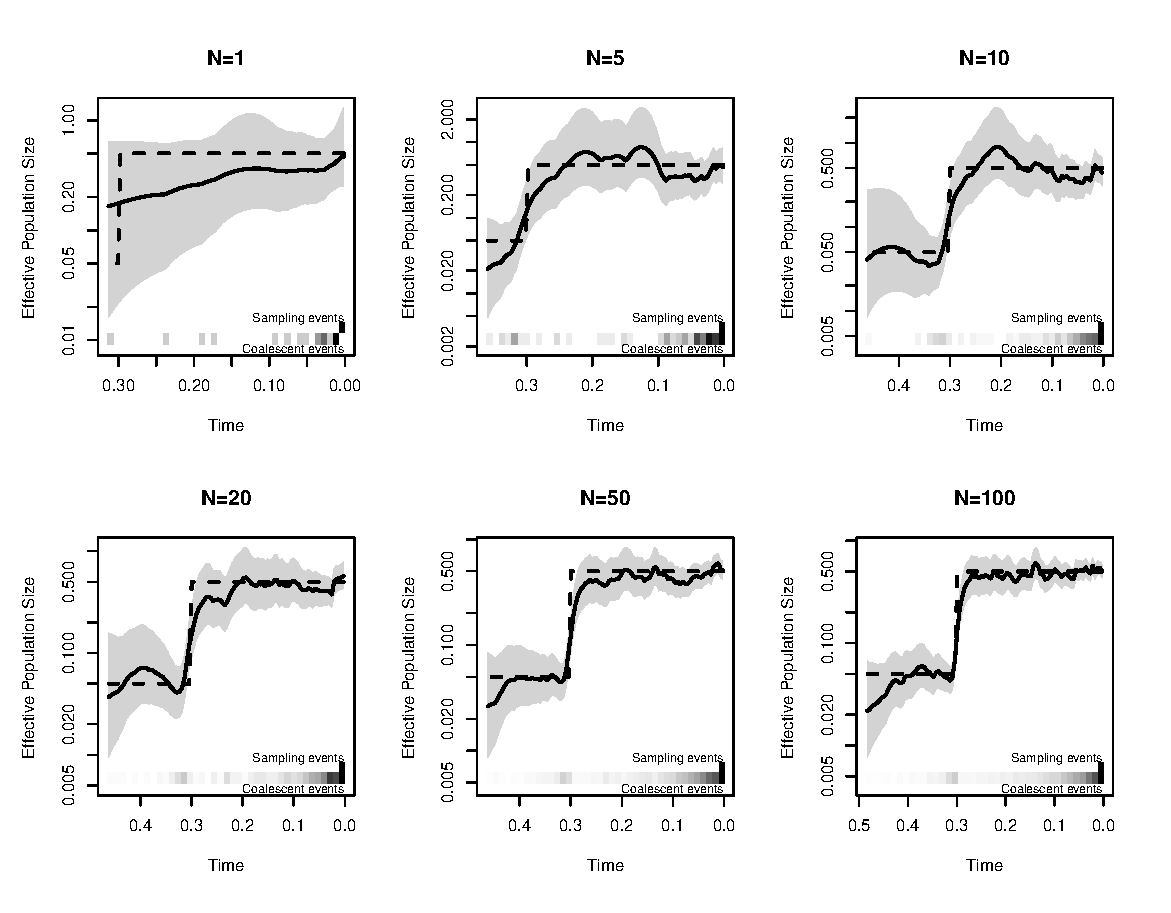
\includegraphics[scale=0.8]{Figures/Bottle_20_independent.eps}    \end{center}
      \caption{\small{INLA-based inference of $N_{e}(t)$ from $N=1$ to $N=100$ independent genealogies simulated under a population bottleneck (dashed line). Posterior median is represented by a solid black line and 95\% BCIs are represented by the shaded areas. Increasing the number of independent genealogies improves inference.}}

\end{figure}
 
%\subsection*{Inferring Ne from sequential local genealogies}
%This is the SMC implementation.
% I decided not to include this code in this package


%\subsection*{New coalescent simulators}
%\citep{Palacios2013}

%\subsection*{More functions}
%\citep{Hein2005}


\subsection*{Implementation of Wright-Fischer estimators}
% Perhaps insert wordage from Wright-Fischer intro into here? See also Christine's comments on intro

Wright-Fischer estimators calculate $N_e$ of a population over the past few generations, whereas coalescent estimators generally integrate $N_e$ over the past $N_e$ to $4*Ne$ generations, depending of the mode of inheritance of the genetic marker employed. They generally summarize the genetic data at hand, and estimate $N_e$ when mutation rates are known, else its mutation-rate scaled counterpart $\theta$. The \texttt{R}-package \texttt{ape} provides functions to calculate $\theta$ based on levels of homozygosity, the number of segregating sites, or the expected number of alleles \citep{Paradis2004}. The \texttt{R}-package \texttt{NB} implements a likelihood estimator based on observed magnitude of genetic drift between generations, called temporal effective population size. Unfortunately, it is not straightforward to generate the required data input format. While other programs have implemented calculations based on levels of linkage disequilibrium, this is the first time to our knowledge that they has been implemented in an \texttt{R}-package. To facilitate comparisons across multiple estimators, it is desirous to keep calculations in the same platform to prevent error.

\subsubsection*{Temporal effective population size}

Temporal $N_e$, also called variance $N_e$, is based on the premise that finite populations experience genetic drift. This drift results in random changes in allele frequencies from one generation to the next which are inversely proportional to $N_e$ \citep{Nei1981}. To implement this method, we need genotypic data from at least one locus sampled during two or more generations (assumed to be non-overlapping).  Given a set of loci sampled from known generations, the \texttt{varNE} function will calculate the point estimate for $N_e$ for each possible comparison. Confidence intervals are obtained using jackknifing. 
%However, for many systems, obtaining samples across multiple generations may be unrealistic.

\subsubsection*{Linkage Disequilibrium}

We also implement a method to calculate $N_e$ based on the magnitude of linkage disequilibrium (LD). Generally, smaller populations are expected to give rise to higher LD than larger populations. 
\cite{Waples2006} demonstrated that low frequency alleles will bias estimates of $N_e$. Therefore, we specify the lowest allele frequency to be retained in the dataset.  While \cite{Waples2008} suggest critical values between 0.05 and 0.01, this value is dataset dependent and we leave it to the user to determine the proper cut-off. The \texttt{LDNe} function requires users to characterize their system as mating randomly, or monogamously. In most cases, random mating may be more appropriate, as it refers to the lifetime mating pattern. 

%\subsection{Existing Ne estimators in R}
%NB package is a multiple sample maximum likelihood estimator\citep{Hui2014}.
%CES: I incorporated this into the intro section to "implementation of Wright-Fischer estimators"

%\subsection{Potential applications}
%Combine with phangorn to full coalescent-based inference from sequence data.
%Combine all Wright fischer estimators into single wrapper function 
%Approximate Bayesian Computation method to calculate Wright FIscher Ne

\bibliography{multiNE}
\end{document}
